\section{GoogLeNet}

We chose GoogLeNet as our team-name in the ILSVRC14 competition. This name is an homage to Yann LeCun’s pioneering LeNet 5 network~\cite{lecun1989backprop}. We also use GoogLeNet to refer to the particular incarnation of the Inception architecture used in our submission for the competition. We have also used a deeper and wider Inception network, the quality of which was slightly inferior, but adding it to the ensemble seemed to improve the results marginally. We omit the details of that network, since our experiments have shown that the influence of the exact architectural parameters is relatively minor. Here, the most successful particular instance (named GoogLeNet) is described in Table \ref{googlenet} for demonstrational purposes. The exact same topology (trained with different sampling methods) was used for 6 out of the 7 models in our ensemble.

\begin{table}
{\tiny
\begin{tabular}[H]{|l|c|c|c|c|c|c|c|c|c|c|c|}
\hline
{\bf type} & {\bf \stackanchor{patch size/}{stride}} & {\bf \stackanchor{output}{size}} & 
{\bf depth} & {\bf $\#1{\times}1$} & {\bf \stackanchor{$\#3{\times}3$}{reduce}} & $\#3{\times}3$ & 
{\bf \stackanchor{$\#5{\times}5$}{reduce}} & $\#5{\times}5$ & {\bf \stackanchor{pool}{proj}} & 
{\bf params} & {\bf ops} \\
\hline\hline
convolution & $7{\times}7/2$ & $112{\times}112{\times}64$ & 1 & & & & & & & 2.7K & 34M \\
\hline
max pool & $3{\times}3/2$ & $56{\times}56{\times}64$ & 0 & & & & & & & & \\
\hline
convolution & $3{\times}3/1$ & $56{\times}56{\times}192$ & 2 & & 64 & 192 & & & & 112K & 360M \\
\hline
max pool & $3{\times}3/2$ & $28{\times}28{\times}192$ & 0 & & & & & & & & \\
\hline
inception (3a) & & $28{\times}28{\times}256$ & 2 & 64 & 96 & 128 & 16 & 32 & 32 & 159K & 128M \\
\hline
inception (3b) & & $28{\times}28{\times}480$ & 2 & 128 & 128 & 192 & 32 & 96 & 64 & 380K & 304M \\
\hline
max pool & $3{\times}3/2$ & $14{\times}14{\times}480$ & 0 & & & & & & & & \\
\hline
inception (4a) & & $14{\times}14{\times}512$ & 2 & 192 & 96 & 208 & 16 & 48 & 64 & 364K & 73M \\
\hline
inception (4b) & & $14{\times}14{\times}512$ & 2 & 160 & 112 & 224 & 24 & 64 & 64 & 437K & 88M \\
\hline
inception (4c) & & $14{\times}14{\times}512$ & 2 & 128 & 128 & 256 & 24 & 64 & 64 & 463K & 100M \\
\hline
inception (4d) & & $14{\times}14{\times}528$ & 2 & 112 & 144 & 288 & 32 & 64 & 64 & 580K & 119M \\
\hline
inception (4e) & & $14{\times}14{\times}832$ & 2 & 256 & 160 & 320 & 32 & 128 & 128 & 840K & 170M \\
\hline
max pool & $3{\times}3/2$ & $7{\times}7{\times}832$ & 0 & & & & & & & & \\
\hline
inception (5a) & & $7{\times}7{\times}832$ & 2 & 256 & 160 & 320 & 32 & 128 & 128 & 1072K & 54M \\
\hline
inception (5b) & & $7{\times}7{\times}1024$ & 2 & 384 & 192 & 384 & 48 & 128 & 128 & 1388K & 71M \\
\hline
avg pool & $7{\times}7/1$ & $1{\times}1{\times}1024$ & 0 & & & & & & & & \\
\hline
dropout (40\%) & & $1{\times}1{\times}1024$ & 0 & & & & & & & & \\
\hline
linear & & $1{\times}1{\times}1000$ & 1 & & & & & & & 1000K & 1M \\
\hline
softmax & & $1{\times}1{\times}1000$ & 0 & & & & & & & & \\
\hline
\end{tabular}
}
\caption{GoogLeNet incarnation of the Inception architecture}
\label{googlenet}
\end{table}

All the convolutions, including those inside the Inception modules, use rectified linear activation. The size of the receptive field in our network is $224{\times}224$ taking RGB color channels with mean subtraction. ``$\#3{\times}3$ reduce'' and ``$\#5{\times}5$ reduce'' stands for the number of $1{\times}1$ filters in the reduction layer used before the $3{\times}3$ and $5{\times}5$ convolutions. One can see the number of $1{\times}1$ filters in the projection layer after the built-in max-pooling in the “pool proj” column. All these reduction/projection layers use rectified linear activation as well.

\begin{figure}
\centering
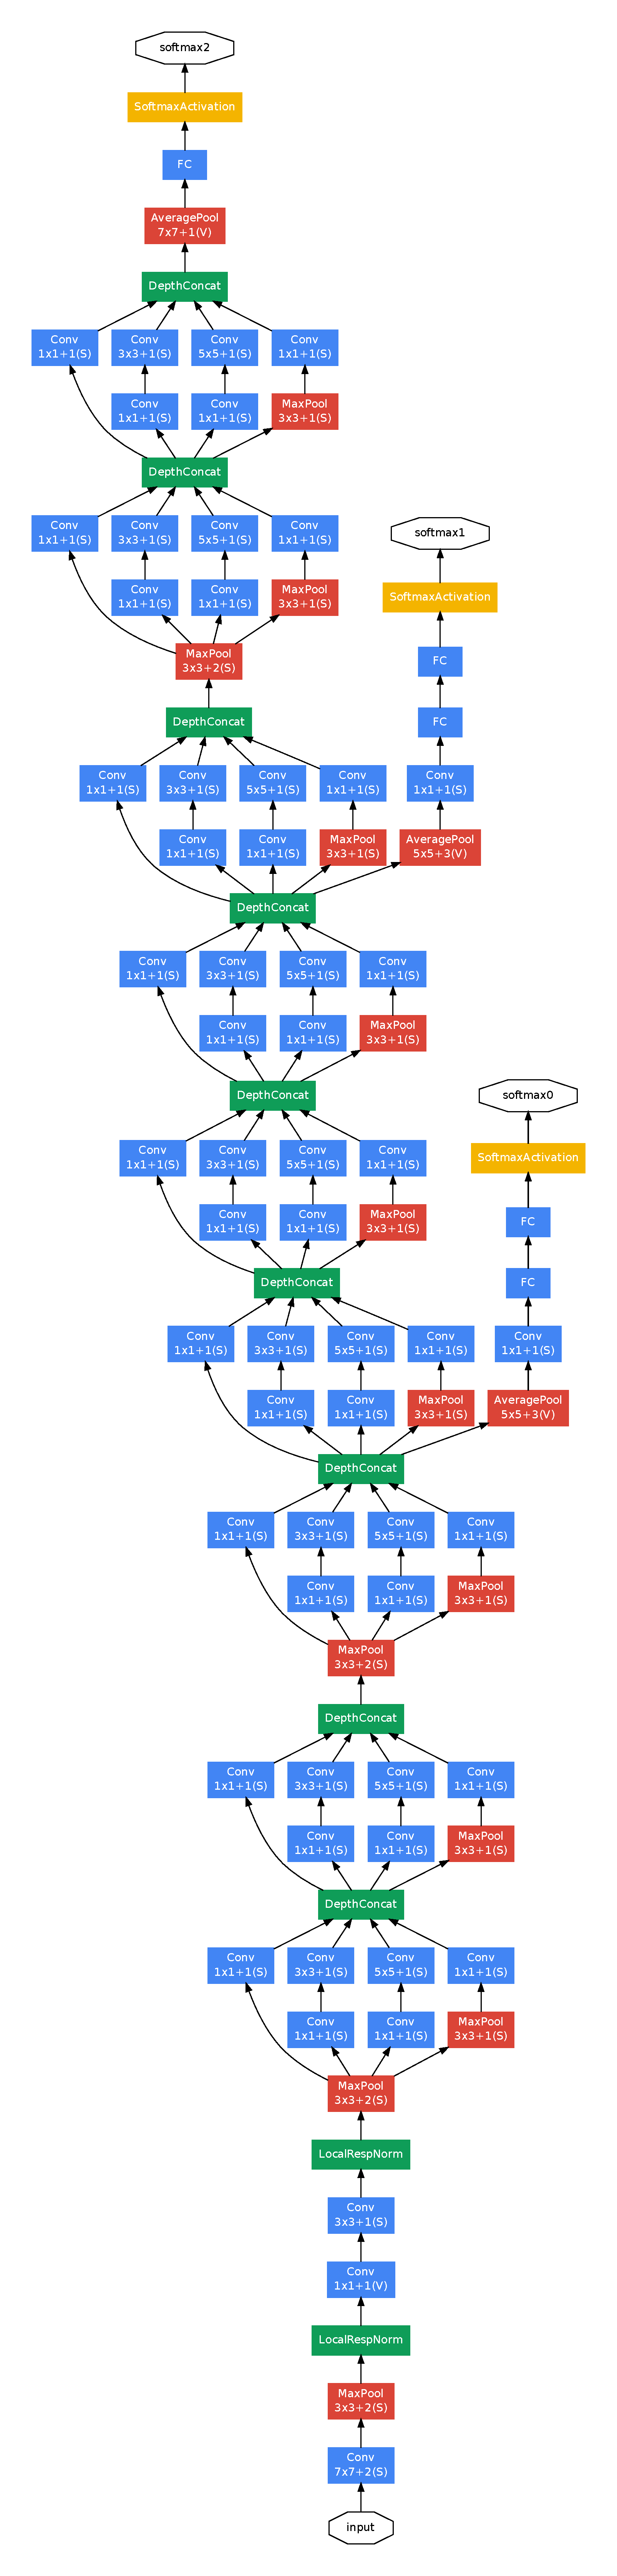
\includegraphics[width=0.38\textwidth]{inceptionoverall.pdf}
\caption{GoogLeNet network with all the bells and whistles}
\label{fig:googlenet}
\end{figure}

The network was designed with computational efficiency and practicality in mind, so that inference can be run on individual devices including even those with limited computational resources, especially with low-memory footprint. The network is 22 layers deep when counting only layers with parameters (or 27 layers if we also count pooling). The overall number of “layers” (independent building blocks) used for the construction of the network is about 100. However this number depends on the machine learning infrastructure system used. The use of average pooling before the classifier is based on \cite{lin2013nin}, although our implementation differs in that we use an extra linear layer. This enables adapting and fine-tuning our networks for other label sets easily, but it is mostly convenience and we do not expect it to have a major effect. It was found that a move from fully connected layers to average pooling improved the top-1 accuracy by about 0.6\%, however the use of dropout remained essential even after removing the fully connected layers.

Given the relatively large depth of the network, the ability to propagate gradients back through all the layers in an effective manner was a concern. One interesting insight is that the strong performance of relatively shallower networks on this task suggests that the features produced by the layers in the middle of the network should be very discriminative. By adding auxiliary classifiers connected to these intermediate layers, we would expect to encourage discrimination in the lower stages in the classifier, increase the gradient signal that gets propagated back, and provide additional regularization. These classifiers take the form of smaller convolutional networks put on top of the output of the Inception (4a) and (4d) modules. During training, their loss gets added to the total loss of the network with a discount weight (the losses of the auxiliary classifiers were weighted by 0.3). At inference time, these auxiliary networks are discarded.

The exact structure of the extra network on the side, including the auxiliary classifier, is as follows:
\begin{itemize}
\item An average pooling layer with $5{\times}5$ filter size and stride $3$, resulting in an $4{\times}4{\times}512$ output for the (4a), and $4{\times}4{\times}528$ for the (4d) stage.
\item A $1{\times}1$ convolution with 128 filters for dimension reduction and rectified linear activation.
\item A fully connected layer with 1024 units and rectified linear activation.
\item A dropout layer with 70\% ratio of dropped outputs.
\item A linear layer with softmax loss as the classifier (predicting the same 1000 classes as the main classifier, but removed at inference time). 
\end{itemize}

A schematic view of the resulting network is depicted in Figure~\ref{fig:googlenet}.
